\documentclass[tikz,border=12pt]{standalone}
\begin{document}
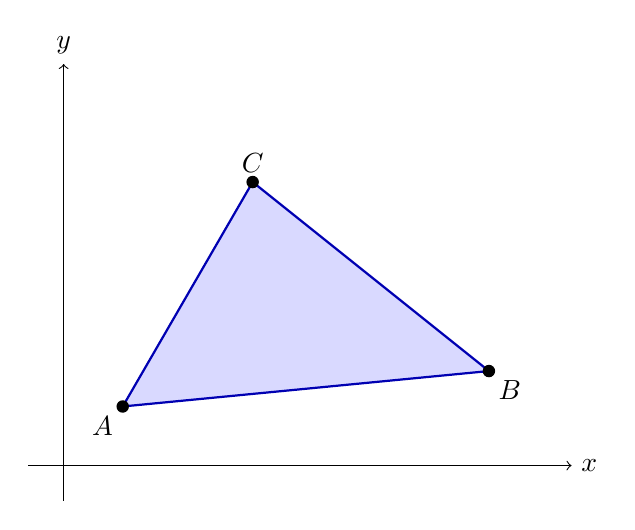
\begin{tikzpicture}[scale=1.5]
\draw[->] (-0.3,0) -- (4.3,0) node[right] {$x$};
\draw[->] (0,-0.3) -- (0,3.4) node[above] {$y$};
\coordinate (A) at (0.5,0.5);
\coordinate (B) at (3.6,0.8);
\coordinate (C) at (1.6,2.4);
\fill[blue!15] (A) -- (B) -- (C) -- cycle;
\draw[thick, blue!70!black] (A) -- (B) -- (C) -- cycle;
\fill (A) circle (1.5pt) node[below left] {$A$};
\fill (B) circle (1.5pt) node[below right] {$B$};
\fill (C) circle (1.5pt) node[above] {$C$};
\end{tikzpicture}
\end{document}
